\section{Simulator}
\label{chap:4}

This section presents the structure of the simulator and a brief tutorial ``\textbf{How to use my project}". The simulator was written in Elixir 1.3. Elixir is a dynamic functional programming language designed for building fault tolerant, scalable and maintainable application. Elixir is based on Erlang virtual machine Beam, widely used for building fault tolerant distributed systems. The project includes a topology generator written in python. The topology generator is an open source implementation under MIT license that was customised for this project. The original code can be found here \url{https://github.com/tcoyze/stochastic-blockmodel}. The repository of the full project can be found in \url{https://github.com/mtileria/SymmetryBreaking} including the modified topology generator. The graphs were plotted using the language R.



\subsection{Simulator Structure}

The simulator is based on the Actor model for concurrent systems. In Elixir, all programs run inside a lightweight process that is isolated from others and it can only communicate via messages. Regarding the \textit{MIS} algorithm implementation, there is a mapping from the graph to the processes. Every vertex of the graph is associated with an elixir process that runs the same distributed algorithm. The communication channel among processes represents the edges of the graph.   

\textbf{Mix} is an Elixir tool for creating, compiling and testing applications. This tool was used to create the project template. In the simulator directory, the sub directory \textbf{config} is created by default and contain the project configurations.  The implementation of the algorithm are in the \textbf{lib} directory, which has 3 sub directories (\textbf{global}, \textbf{alpha} and \textbf{beta}), one for each synchronisation technique  .

The complete project structure is presented below. The two main directories are ``\textbf{generator}" and ``\textbf{simulator}". The code related to the synchronous simulation and \textit{MIS} are in the simulator directory while the topology generator is in the generator directory. 


\begin{verbatim}
SymmetryBreaking/
|
|--generator
|  |-- graph
|  |-- topologies
|  main.py
|--simulator
|  |-- config
|  |-- files
|  |-- lib
|      |-- beta
|           |-- Beta.ex
|           |-- sync_mis_beta.ex
|           |-- b_controller.ex
|      |-- alpha
|           |-- alpha.ex
|           |-- sync_mis_alpha
|           |-- a_controller.ex
|      |-- global
|           |-- g_mis.ex
|           |-- g_controller.ex
|  |--results
|  |--test
\end{verbatim}

\subsection{MIS with Global Synchronizer}
 
The implementation of the \textit{MIS} algorithm with the global synchronizer is in the directory \textbf{simulator/lib/global}. The \textbf{MIS} algorithm is in the file \textbf{g\_mis.ex} and file \textbf{g\_controller.ex} contains the module \textbf{GlobalSync} which handle the start and finish of the simulation, also the synchronisation mechanism. 

In the \textbf{GlobalSync} module, the function \textit{start\_nodes n} is the start point of the simulation, where \textbf{n} is the number of processes to be spawned. This function is in charge of spawn the processes that are going to run the \textit{MIS} algorithm, henceforth active processes. The first task of this function is to spawn the master process, which is the one that it is going to indicate actives processes when to start the algorithm.  Besides that, the master process controls when a new round starts and receives the output of the processes at the end of the algorithm, the output will be for the \textit{MIS} algorithm \textbf{:mis\_member} or \textbf{:not\_mis\_member}. 

Actives processes are spawned according to the information in the files  \textbf{N\_nodes.txt} and \textbf{N\_edges.txt}. These files are generated previously with the topology generator. The adjacency's of each vertex is read from another file and the list of neighbours is sent to each active process. The implementation for the global simulation is described with details showing the most important part of the code. Similar details are omitted in the description of the Alpha and Beta implementation. A \textit{start\_nodes n} is illustrated below.


\begin{lstlisting}[frame=single, columns=fullflexible, mathescape=true, caption= start\_nodes function, label = code:start]


def start_nodes (n) do
  master_id = spawn(GlobalSync,
  :run_master,[GlobalSync.init_master(n)])
  case :global.register_name(:master,master_id) do
    :yes -> master_id
    :no -> :error
  end

  stream = File.stream!("N_nodes.txt")
  p_names = String.split(List.first(Enum.take stream,1))
  p_ids = for name <- p_names do
    pid = spawn(MIS,:run, [MIS.init_state(name,
    master_id)])
    case :global.register_name(name,pid) do
      :yes ->
        pid
      :no -> :error
    end
  end
  send(master_id,{:add_processes_list,p_ids})
  add_edges_topology(n)
end
\end{lstlisting}


Once the master process had created $N$ processes, it remains waiting for the arrival of messages send by active processes in a recursive function named \textbf{run\_master(state)}. The variable \textbf{state} keeps the information about the simulation, for instance, message counter, actives processes, actual round, among other data.

 The construction \textbf{receive do} indicate a process that  it should be waiting for messages that match with specified patterns, in the form of $\{:pattern\} \rightarrow$. When a process receives any message, it does a pattern matching against all specified options and executes the code of the first pattern that matches. To illustrate the concept, the pattern \textit{:update\_complete} is used by the master process to receive the notification of active processes after the computing for one round is finished and pattern \textit{:kill\_all} send a message indicating processes to finish the simulation. 

\begin{lstlisting}[frame=single, columns=fullflexible, mathescape=true, caption= run\_master function for master, label = code:run]
def run_master(state) do
state =
  receive do

    {:start_mis} ->
      Enum.each(state.processes, fn(pid) ->
        send(pid,{:find_mis,:initial})end)
      state

    {:update_complete} ->
      if state.count_topology == state.active_size do
         state = $\%${state | count_topology: 0}
         next_round = state.actives
         state = $\%${state | actives: []}
         Enum.each(next_round, fn(pid) -> 
            send(pid,{:find_mis,:continue})end)
         state
      end
        
    {:kill_all} ->
      Enum.each(state.processes, fn(x) -> send x,{:kill} end)
      Process.exit(self, :exit)
      
  end
  run_master(state)
end

\end{lstlisting}

The code \ref{code:output} shows the steps that take the master process when active processes finish the execution of one round. The master process keeps waiting for messages until the number of processes that have sent the message is equal to the number of active processes, meaning that the round is finished. The master process split the network in processes that are part of the \textit{MIS} and the ones that are still active.  Finally, if there are still active processes, then send a message indicating to continue with the next round of the algorithm, in another case, the distributed algorithm has ended.   
 
 
\begin{lstlisting}[frame=single, columns=fullflexible, mathescape=true, caption= Output of processes per round  , label = code:output]
{:complete,mis,active,sender,msg_count} ->
  state = $\%${state | count: state.count + 1}
  {num_msg,sync_overhead} = update_message_counter
    (state.msg_counter,msg_count,state.round)
  state = put_in(state, [:msg_counter,state.round],
    {num_msg,sync_overhead})

state =
    cond  do
    active == false && mis == true ->  
      state = $\%${state | mis: state.mis ++ [sender]}
    active == false && mis == false ->
      state = $\%${state | to_delete: state.to_delete + 1}
    true ->  
      state = $\%${state | actives: state.actives ++ [sender]}
    end

if state.count == state.active_size do
    IO.puts(ROUND FINISH)
    <@\textcolor{green}{\#safe results for round}@> 
    
    case state.active_size == 0 do
      true ->
        IO.puts(MIS complete)
        <@\textcolor{green}{\#save results for algorithm}@> 
        state
       false ->
        <@\textcolor{green}{\# continue next round for active processes}@> 
        Enum.each(state.actives, fn(pid) ->
        send(pid,{:update_topology})end)
        state
end
\end{lstlisting}


The \textbf{MIS} module, in the \textbf{g\_mis.ex} file has the implementation of the algorithm. The module follows the same logic as the global synchronizer. There is a state of the algorithm and a function named \textbf{run(state)} that is running recursively waiting to receive messages. If a message matches the pattern $\{:find\_mis\}$, a random value is selected and the process $p_i$ send this value to its neighbours. This messages is received by $p_j$ with the pattern $\{:value\}$. If the value generated of $p_i$ is the smaller of its neighbour's values, then $p_i$ is part of the $MIS$.  

For every message $p_i$ send an acknowledge message $\{:ack\}$, and when $p_i$ has received the acknowledgement for all its neighbours, then send a $\{:safe\}$ message to each neighbour. Again, when $p_i$ has received a  $\{:safe\}$ message from all its neighbours, inform the master process that it has complete the computation for the current round. The partial implementation of the \textbf{run(state)} is shown in the code \ref{code:run_global}.

\begin{lstlisting}[frame=single, columns=fullflexible, mathescape=true, caption= run function for \textit{MIS} , label = code:run_global]

def run(state) do


 state = receive do

   {:find_mis,x} ->  

   {state | value: :rand.uniform()}
      Enum.each(state.neighbours, fn (node) ->
      send(node,{:value,state.value,my_pid})end)
      state


   {:value,value,sender,} ->
    state = $\%${state | n_receive: state.n_receive + 1}
    state = if (state.value < value),
     do: state = $\%${state | count: state.count + 1} 
    if state.n_receive == state.n_size do
     case state.count == state.n_size do
       true->  
        state = $\%${state | mis: true}
       false ->
         state = $\%${state | n_receive: 0}
    end
    send(sender,{:ack})
    state

   {:ack} ->
    state = $\%${state | ack: state.ack + 1}
    if state.ack == state.n_size do
      notify_neighbours(state.neighbours,{:safe})
     end
    state

   {:safe,neighbour_mis} ->
    state = $\%${state | safe_count: state.safe_count + 1}
     if state.safe_count == state.n_size do
       send(state.master_id,{:complete)
     end
    state
    
   run(state)

\end{lstlisting}

\subsection{MIS with Alpha Synchronizer}

The \textit{MIS} implementation with the Alpha Synchroniser is slightly different. The module \textbf{Controller} in the file \textbf{a\_controller} is the one in charge of creating the master and actives processes, start the algorithm, control the rounds and store the output state of processes. For the Alpha Synchronizer there is no \textbf{:update\_topology} message because inactive processes remain sending ``dummy'' to keep the synchronization mechanism.


When $p_i$ is spawned, also the synchronizer $alpha_i$ is spawned and a link is created between $alpha_i$ and $p_i$, this is shown in the code \ref{code:alpha_start}.  Implementing the synchronisation and the algorithm in different processes allows any other algorithm to use the synchronous simulation. 

\begin{lstlisting}[frame=single, columns=fullflexible, mathescape=true, caption= start function , label = code:alpha_start]
def start(name,master) do
  alpha = Alpha.start(name)
  pid = spawn(SyncMIS,:run, [init_state(name,master,alpha)])
  send(alpha,{:main_process,pid})
  case :global.register_name(name,pid) do
    :yes -> pid
    :no  -> :error
  end
end

\end{lstlisting}



The \textbf{sync\_mis\_alpha} implement the module for the \textit{MIS} algorithm. The functions \textbf{sync\_send(synchronizer,msg)} and \textbf{sync\_recv(round,msg)} provide the interfaces to interact with the synchronizer. Any synchronous algorithm can use Alpha calling these functions. The function are illustrated in the code \ref{code:send_recv}.

\begin{lstlisting}[frame=single, columns=fullflexible, mathescape=true, caption= Interface for synchronise send and receive, label = code:send_recv]

def sync_send(synchronizer,msg) do
  send(synchronizer,{:sync_send,msg})
end

def enable_sync_recv(pid, round, buffer,type) do
  send(pid,{:sync_rcv,type,buffer})
end

\end{lstlisting}


When $p_i$ call the \textbf{sync\_send} function, a message is sent to $alpha_i$ containing the messages for a new round. For every round, once $alpha_i$ has received all messages from each $alpha_j$ such $p_j$ is a neighbour of $p_i$, it call the \textbf{sync\_recv} function in order to send to $p_i$ the mesaages store in the buffer. In consequence, $p_i$ receive all messages together for each round.  The code \ref{code:sync_call} shows how the \textbf{MIS} algorithm uses the interfaces for the synchronous simulation. The module Alpha implement the algorithm \ref{algorithm:alpha} explained is section \ref{chap:3}.

\begin{lstlisting}[frame=single, columns=fullflexible, mathescape=true, caption= Synchronous communication by \textit{MIS} algorithm, label = code:sync_call]

{:find_mis,x,_} ->  # x = :continue || :initial
    state = $\%${state | value: :rand.uniform()}
    sync_send(state.synchronizer_id,{:value,state.value})
    state
{:sync_recv,:value,_,buffer} ->
    state = $\%${state | step: :recv_value}
    is_min = Enum.all?(buffer,fn {_,y} -> state.value < y end)
    state =
      case is_min do
        true ->
          state = $\%${state | mis: true}
        false ->
          state
       end
    sync_send(state.synchronizer_id,{:mis_status,state.mis})
    state

\end{lstlisting}

\subsection{MIS with Beta Synchronizer}

The implementation of the \textit{MIS} algorithm with the Beta Synchronizer is very similar to the implementation with the Alpha. The main difference is the initialisation phase that has to be done with Beta. Before $p_i$ call the function \textbf{run(state)}, every active processes execute the \textbf{pre\_run(state)} function to construct the rooted spanning tree. The master process chooses a random process to act as a root and this process starts the construction of the spanning three sending a message \textbf{{:construct,:rst,my\_pid}} to every neighbour. The first time $p_i$ receive the message reply to the sender $p_j$ with a \textbf{:parent} message and set the parent to the $p_j$ in its state. In another case, reply with a \textbf{:reject} message to $p_j$. Once all processes are part of the spanning tree, the topology is ready to run any algorithm. The \textit{pre\_run} function is shown in the code \ref{code:spanningtree}.


\begin{lstlisting}[frame=single, columns=fullflexible, mathescape=true, caption= Spanning Tree construction in Beta, label = code:spanningtree]

state = receive do

  {:spanning_tree,:root} ->
     Enum.each(Map.keys(state.neighbors),
       fn(dest) -> send dest,{:construct,:rst,my_pid} end)
 	 state

  {:search,:rst,origin} ->
 	if state.parent == nil do
 	   state = $\%${state | parent: origin}
 	   send origin,{:reply,:parent_of, my_pid}
       Enum.each(state.neighbors  -- [origin],
       fn dest -> send dest,{:search,:rst,my_pid} end)
 	else
 	   send origin, {:reply,:rejected, my_pid}
 	end
    state

 {:reply, value, origin} ->
    state = $\%${state | replies: state.st_replies - 1}
     state =
     if value == :parent_of, do:  
        state = $\%${state | childs:state.childs ++ [origin]
     if state.st_replies == 0 do
 	     run(state)
    end
 	state
    

\end{lstlisting}



\subsection{How to use my program}

The only requirement to run the simulator is to have installed Elixir. The Erlang virtual machine is in charge of handle the interaction with the operating system, so there are no special requirements for the platform. The following example was running on a Debian base operating system, however, the same steps will work on any Windows or Mac operating system.     

This tutorial show the steps to use the simulator assuming that the user will start from scratch. The first step is to download the simulator from the repository in github. This can be done installing git or simply downloading the project from the web page \url{https://github.com/mtileria/SymmetryBreaking.git}. The command is for clone the project is:

\begin{lstlisting}[language=bash, columns=fullflexible,mathescape=true]
   $ \$$ git clone https://github.com/mtileria/SymmetryBreaking.git
\end{lstlisting}

After the project is locally store, one may choose which simulation execute. This can be done in many ways in Elixir. This example shows how to compile and execute manually using the Elixir interactive shell \textbf{iex}. The user have to navigate to the specific simulator directory, in this example, the sub directory \textbf{alpha}, \textbf{beta} or \textbf{simulator/lib/global}. An example of the steps for compiling and running the \textit{MIS} algorithm with global synchronisation is illustrated below. The image \ref{fig:gmis_run} shows the output of the execution of the simulation for 8192 processes. Once the distributed algorithm is finished, the \textbf{finish\_simulation} function send a \textbf{:kill} message to each process spawned before. This function needs to be call before start another execution. 


\begin{lstlisting}[style=terminal]

marcos@mtileriaPC ~/simulator/lib/global \$ iex
iex(1)> c "GlobalSync.ex"
[GlobalSync]
iex(2)> c "g_mis.ex"     
[MIS]
iex(3)> GlobalSync.start_nodes(8192)
:ok
iex(4)> GlobalSync.start_mis        
start_mis/0    
iex(4)> GlobalSync.start_mis
{:start_mis}


\end{lstlisting}

\begin{figure}[ht]
\centering
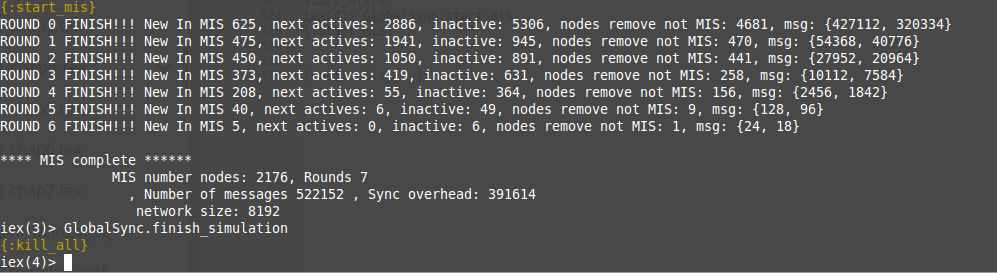
\includegraphics[width=0.9 \linewidth, height=5cm]{g_mis_run.png} 
\caption{Output of the execution of \textit{MIS} algorithm with global synchronizer}
\label{fig:gmis_run}
\end{figure}

To run algorithm using Alpha or Beta synchronizer the steps are similar. For these synchronizers, 3 modules should be compiled before run the algorithm, the module for the master, algorithm and synchronizer processes. The special case is Beta because the rooted spanning tree should be constructed before execute the algorithm. This is done calling the function \textbf{spanning\_tree}. The steps to execute the algorithm with Alpha and Beta are shown in \ref{code:alpha_exe} and \ref{code:beta_exe} respectively.

\begin{lstlisting}[style=terminal,caption= Example of compiling and executing the algorithm with Alpha, label = code:alpha_exe]

marcos@mtileriaPC ~/simulator/lib/alpha \$ iex
iex(1)> c "a_Controller.ex"
[GlobalSync]
iex(2)> c "a_mis.ex"     
[MIS]
iex(2)> c "Alpha.ex"     
[Alpha]
iex(3)> a_controller.start_nodes(8192)
:ok
iex(4)> a_controller.start_mis        
start_mis/0    
{:start_mis}
\end{lstlisting}

\begin{lstlisting}[style=terminal,caption= Example of compiling and executing the algorithm with Beta, label = code:beta_exe]

marcos@mtileriaPC ~/rhul/tesis/lib/beta \$ iex
iex(1)> c "b_Controller.ex"
[GlobalSync]
iex(2)> c "b_mis.ex"     
[MIS]
iex(2)> c "Beta.ex"     
[Alpha]
iex(3)> b_controller.start_nodes(8192)
:ok
iex(4)> b_controller.start_mis        
start_mis/0    
{:start_mis}

\end{lstlisting}

